\documentclass[12pt]{article}
\usepackage[utf8]{inputenc}
\usepackage{graphicx} % Allows you to insert figures
\usepackage{amsmath} % Allows you to do equations
\usepackage{fancyhdr} % Formats the header
\usepackage{geometry} % Formats the paper size, orientation, and margins
\usepackage[style=authoryear-ibid,backend=biber]{biblatex} % Allows you to do citations - does Harvard style and compatible with Zotero
\addbibresource{Example.bib} % Tells LaTeX where the citations are coming from. This is imported from Zotero
\usepackage[english]{babel}
\usepackage{csquotes}
\usepackage{background}
\usepackage{minted}
\renewcommand*{\nameyeardelim}{\addcomma\space} % Adds comma in in-text citations
\linespread{1.5} % About 1.5 spacing in Word
\setlength{\parindent}{0pt} % No paragraph indents
\setlength{\parskip}{1em} % Paragraphs separated by one line
\renewcommand{\headrulewidth}{0pt} % Removes line in header
\geometry{a4paper, portrait, margin=1in}
\setlength{\headheight}{14.49998pt}
\backgroundsetup{scale=1,angle=0,opacity=0.175,contents={
\includegraphics[scale=0.25]{1200px-Vellore_Institute_of_Technology_seal_2017.png}}}


\begin{document}
\begin{titlepage}
\NoBgThispage
   \begin{center}
        \begin{figure}[h] % h - Place the float here, i.e., approximately at the same point it occurs in the source text (however, not exactly at the spot)
        \centering
        
\includegraphics[width=15cm]{1583124354phpJTtnK5.png}
        \end{figure}

        \Huge{Digital Assignment 2}

        \vspace{0.5cm}
        \LARGE{20BIT0406 - Sanchit Sandeep Khedkar}
       
        \vspace{2.5 cm}
        \Large{2022-01-24}
        
        \vspace{0.25 cm}
        \Large{ITE3001 - Data Communication and Computer Networks}
        \large{VL2021220500483 L33+L34}
       

       \vfill
    \end{center}
\end{titlepage}
\newpage

\setcounter{page}{2}
\pagestyle{fancy}
\fancyhf{}
\rhead{\thepage}

Q1.  
Implement a TCP based server program to authenticate the client’s User Name and Password. The validity of the client must be sent as the reply message to the client and display it on the standard output.

Ans- \\ Code- \\ tcpUsernamePasswordValidationServer.py-\inputminted{python}{tcpUsernamePasswordValidationServer.py}
tcpUsernamePasswordValidationClient.py- \inputminted{python}{tcpUsernamePasswordValidationClient.py}
Output-
\begin{figure}[h] % h - Place the float here, i.e., approximately at the same point it occurs in the source text (however, not exactly at the spot)
\centering
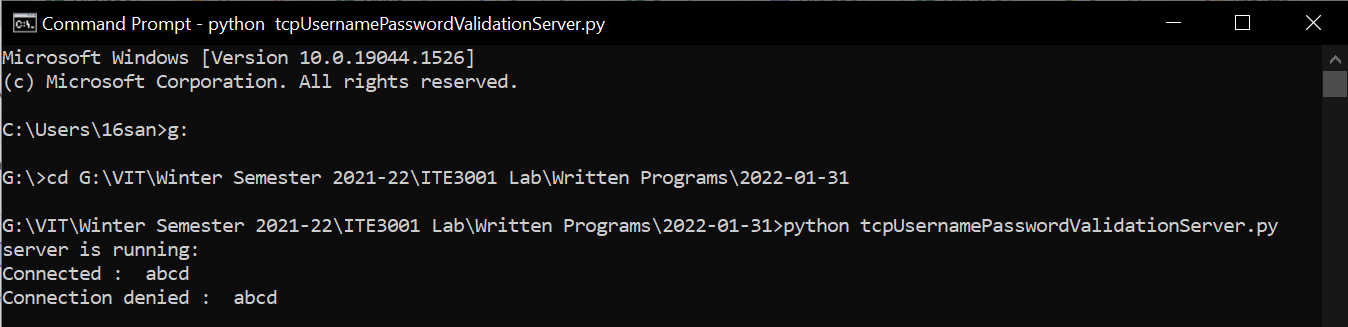
\includegraphics[width=\textwidth]{tcpUsernamePasswordValidationServer.png}
\caption{Server output}
\end{figure}
\begin{figure}[h] % h - Place the float here, i.e., approximately at the same point it occurs in the source text (however, not exactly at the spot)
\centering
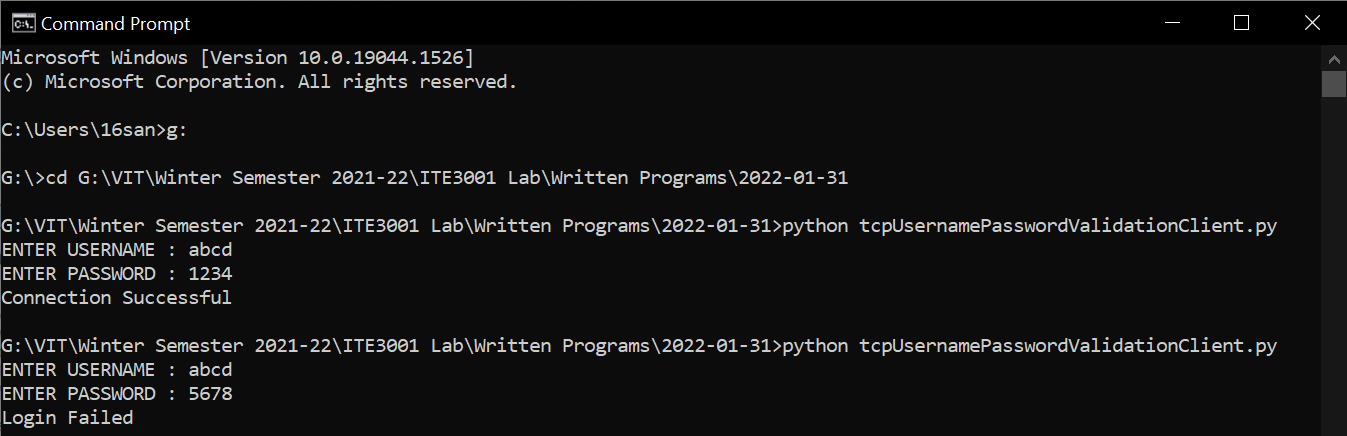
\includegraphics[width=\textwidth]{tcpUsernamePasswordValidationClient.png}
\caption{Client output}
\end{figure}
\newpage

Q2. Write a client server program to detect the errors using simple parity check mechanism. \newline
Ans- \\ Code- \\ tcpSimpleParityServer.py-\inputminted{python}{tcpSimpleParityServer.py}
tcpSimpleParityServer.py- \inputminted{python}{tcpSimpleParityServer.py}
\newpage
Output-
\begin{figure}[h] % h - Place the float here, i.e., approximately at the same point it occurs in the source text (however, not exactly at the spot)
\centering
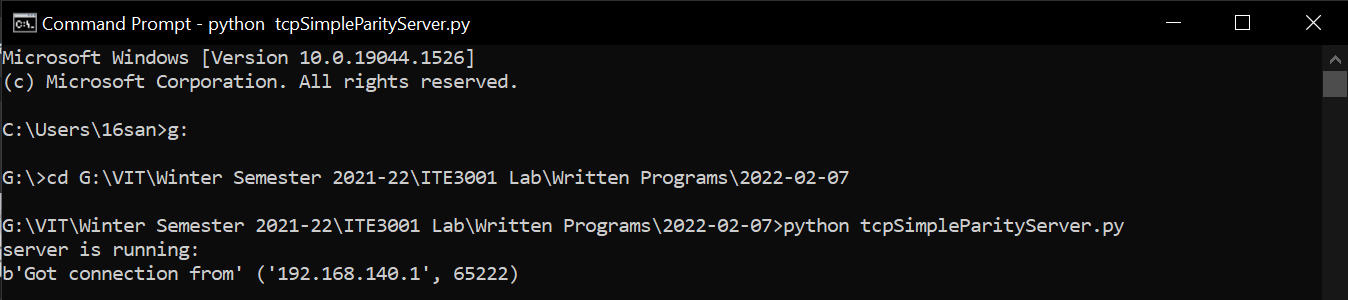
\includegraphics[width=\textwidth]{tcpSimpleParityServer.png}
\caption{Server output}
\end{figure}
\begin{figure}[h] % h - Place the float here, i.e., approximately at the same point it occurs in the source text (however, not exactly at the spot)
\centering
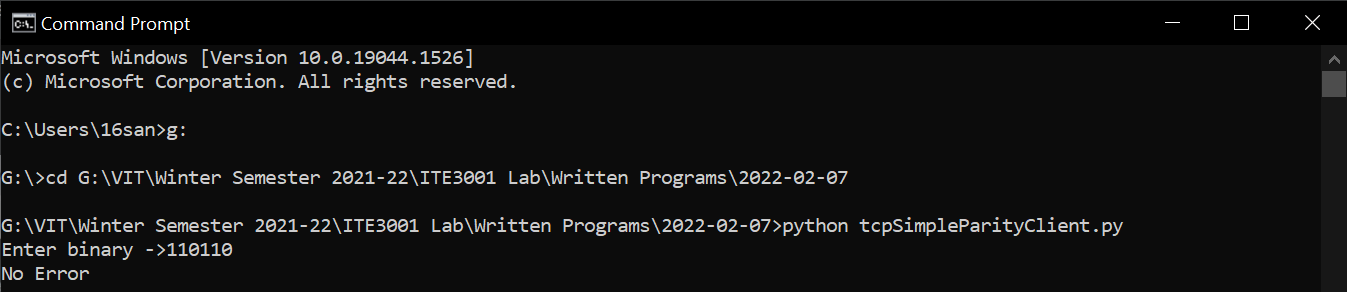
\includegraphics[width=\textwidth]{tcpSimpleParityClient.png}
\caption{Client output}
\end{figure}
\newline

Q3. Write a client server TCP program to correct the errors using hamming code.
a) Only create codeword from the dataword of fixed size (Easy) [50\%]\\
b) Correct the errors of the codeword of a fixed size dataword (Medium) [80\%]\\
c) Correct the errors of the codeword of a dynamic size dataword (Hard) [100\%].\\
Ans- \\ Code (a)- \\ tcpHammingCodeEasyServer.py-\inputminted{python}{tcpHammingCodeEasyServer.py}
tcpHammingCodeEasyClient.py- \inputminted{python}{tcpHammingCodeEasyClient.py}
\newpage
Output-
\begin{figure}[h] % h - Place the float here, i.e., approximately at the same point it occurs in the source text (however, not exactly at the spot)
\centering
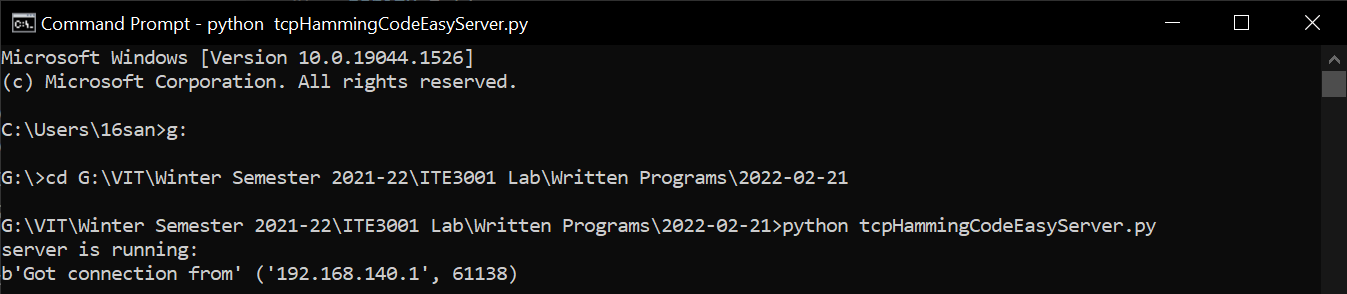
\includegraphics[width=\textwidth]{tcpHammingCodeEasyServer.png}
\caption{Server output}
\end{figure}
\begin{figure}[h] % h - Place the float here, i.e., approximately at the same point it occurs in the source text (however, not exactly at the spot)
\centering
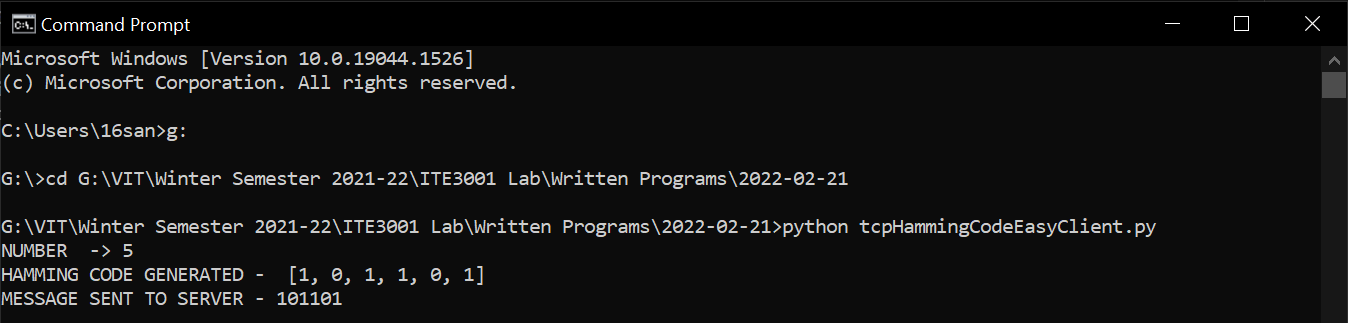
\includegraphics[width=\textwidth]{tcpHammingCodeEasyClient.png}
\caption{Client output}
\end{figure}
\newline
Code (b)- \\ tcpHammingCodeMediumServer.py-\inputminted{python}{tcpHammingCodeMediumServer.py}\\newpage
tcpHammingCodeMediumClient.py- \inputminted{python}{tcpHammingCodeMediumClient.py}
\newpage
Output-
\begin{figure}[h] % h - Place the float here, i.e., approximately at the same point it occurs in the source text (however, not exactly at the spot)
\centering
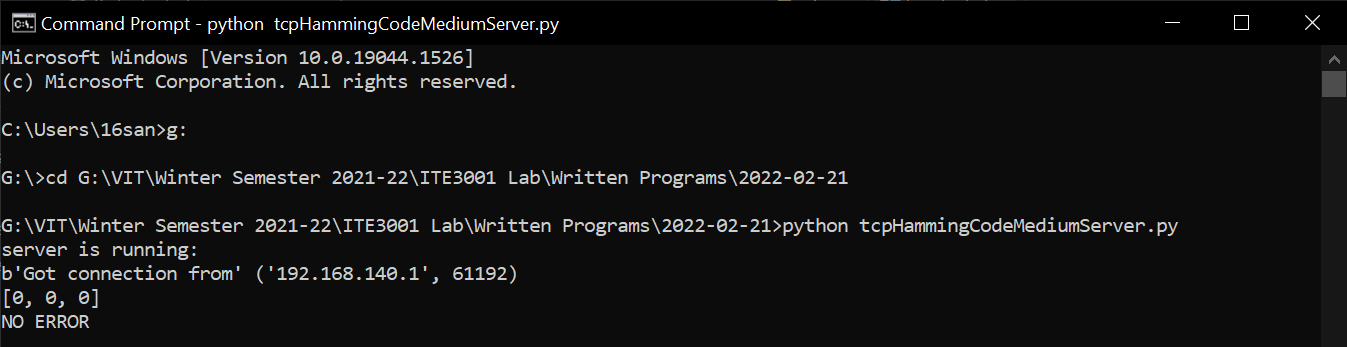
\includegraphics[width=\textwidth]{tcpHammingCodeMediumServer.png}
\caption{Server output}
\end{figure}
\begin{figure}[h] % h - Place the float here, i.e., approximately at the same point it occurs in the source text (however, not exactly at the spot)
\centering
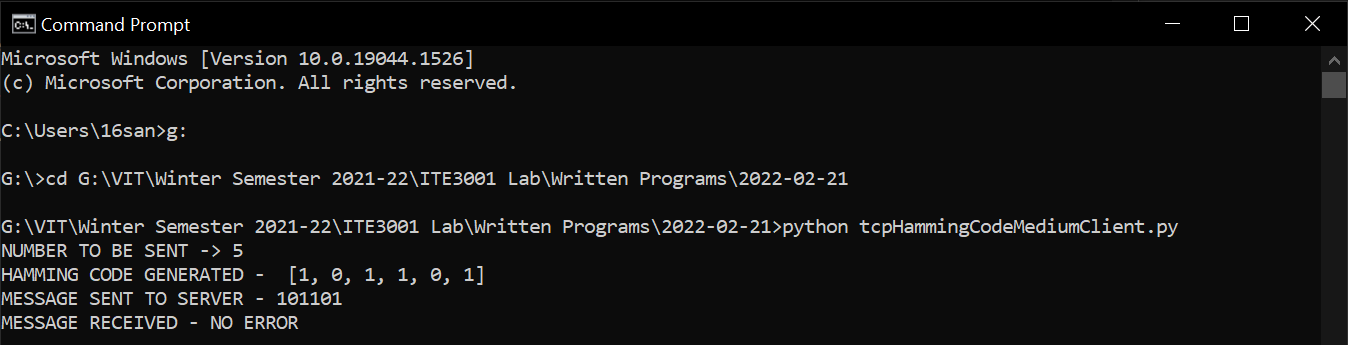
\includegraphics[width=\textwidth]{tcpHammingCodeMediumClient.png}
\caption{Client output}
\end{figure}
\newline
Code (c)- \\ tcpHammingCodeHardServer.py-\inputminted{python}{tcpHammingCodeHardServer.py}
tcpHammingCodeHardClient.py- \inputminted{python}{tcpHammingCodeHardClient.py}
\newpage
Output-
\begin{figure}[h] % h - Place the float here, i.e., approximately at the same point it occurs in the source text (however, not exactly at the spot)
\centering
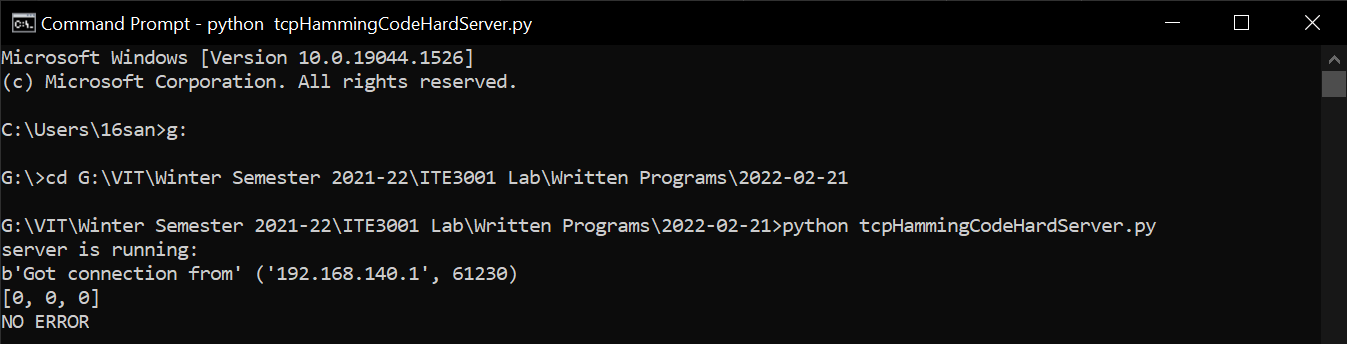
\includegraphics[width=\textwidth]{tcpHammingCodeHardServer.png}
\caption{Server output}
\end{figure}
\begin{figure}[h] % h - Place the float here, i.e., approximately at the same point it occurs in the source text (however, not exactly at the spot)
\centering
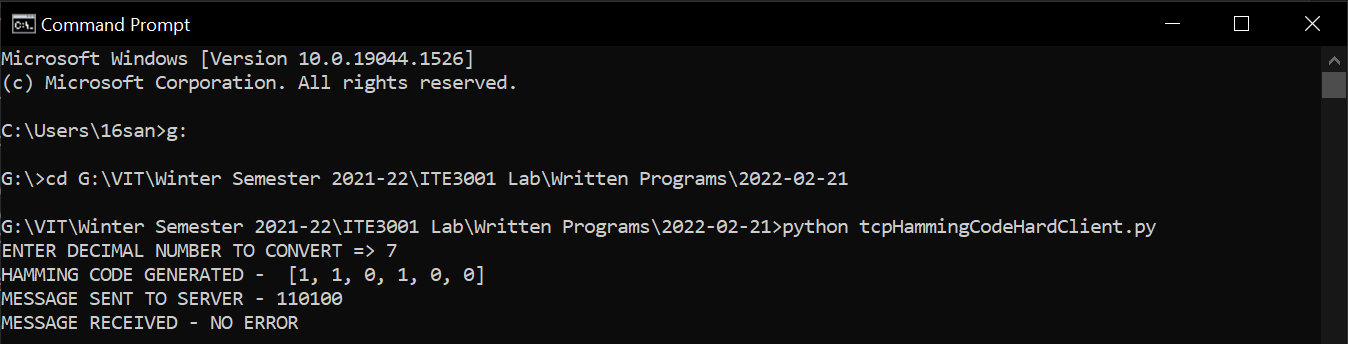
\includegraphics[width=\textwidth]{tcpHammingCodeHardClient.png}
\caption{Client output}
\end{figure}
\end{document}
